%%%%%%%%%%%%%%%%%%%%%%%%%%%%%%%%%%%%%%%%%%%%%%
%%%%%%%%%%%%%%%%%%%%%%%%%%%%%%%%%%%%%%%%%%%%%%
%%% Master Thesis Template by Fabian Schär %%%
%%%%%%%%%%%%%%%%%%%%%%%%%%%%%%%%%%%%%%%%%%%%%%
%%%%%%%%%%%%%%%%%%%%%%%%%%%%%%%%%%%%%%%%%%%%%%

%%%%%%%%%%%%%%%%%%%%%%%%%%%%%%%%%%%%%%
%%% Packages and Document Settings %%%
%%%%%%%%%%%%%%%%%%%%%%%%%%%%%%%%%%%%%%

\documentclass[12pt,a4paper,titlepage,oneside,english]{article}

%%% Main Packages %%%
\usepackage[english]{babel}
%\usepackage[ngerman]{babel} % Use this option for German settings.
\usepackage[T1]{fontenc}
\usepackage[utf8]{inputenc}

%%% Additional Packages %%%
\usepackage{cite}
\usepackage{framed}
\usepackage{graphicx}
%\usepackage[german]{fancyref}
\usepackage[german,hidelinks]{hyperref} %hidelinks
\usepackage{multirow}
\usepackage[round]{natbib}
\usepackage{setspace}
\usepackage{geometry}
\usepackage{pst-all} % Not working with Sweave!!!
\usepackage{tikz}
\usetikzlibrary{positioning, intersections}

%%% Math Packages %%%
\usepackage{amsmath}
\usepackage{amstext}
\usepackage{amssymb}
\usepackage{theorem}
\usepackage{epsfig}
\usepackage{longtable}

%%% Layout Specifications %%%
\geometry{a4paper, top=35mm, left=40mm, right=40mm, bottom=45mm,
headsep=10mm, footskip=12mm}

%%% Parskip Settings %%%
\setlength{\parskip}{3mm}
\setlength{\parindent}{0mm}

%%% Document Specifications %%%
\title{Template Master's Thesis}
\author{John Doe}


%%%%%%%%%%%%%%%%%%
%%% Title Page %%%
%%%%%%%%%%%%%%%%%%

\begin{document}
%\begin{titlepage}
\begin{center}
\vspace{1em}
\large{Master Thesis}\\
\huge Developing Address Clustering Heuristics for Account-Based Blockchain Networks:\\ An Analysis based on a Specific Address Set \\
\Large \vspace{1em}
Dario Thürkauf
\end{center}

\vspace{1em}
\normalsize
\begin{flushleft}
Supervised by:\\ 
Prof. Dr. Fabian Schär \\
Credit Suisse Asset Management (Schweiz) Professor for \\ 
Distributed Ledger Technologies and Fintech \\
Center for Innovative Finance, University of Basel
\end{flushleft}

\vspace{1em}
\onehalfspacing
\begin{center}
\section*{Abstract}
\end{center}
Assentiar consuetae ha opinionum mentemque ob ii. Ne conflantur de intelligat et me cohibendam. Imaginandi ob to at agnoscerem et mutationum. In methodum ob ii at quicquid lectorum. Procuravi ha dependent ob evidenter tangantur concipere. Immortalem objectivus deo eae rei attingebam ita advertebam quamprimum. Typis patet prius qua nia mem ens. Suppono sim ita pendere nam agnosci quopiam vestiri spondeo dum. Tes illum mundo vetus signa fit talem res his.  \\
\vfill
\textbf{Keywords:} Keyword 1, Keyword 2, Keyword 3, Keyword 4.\\
\noindent\textbf{JEL:} X00, X00, X00
%\end{titlepage}


%%%%%%%%%%%%%%%%%%%%%%%%%%%%%
%%% Contents & Declaration%%%
%%%%%%%%%%%%%%%%%%%%%%%%%%%%%

\pagenumbering{gobble}

\newpage
\pagenumbering{Roman}
\tableofcontents

\vfill
\begin{center}

\includegraphics[width=4cm]{../figures/logo_cif.png}
\end{center}
\newpage
\singlespacing
%\vspace{-1.5cm}
\section*{Declaration of Independent Authorship}
I attest with my signature that I have written this work independently and without outside help. I also attest that the information concerning the sources used in this work is true and complete in every respect. All sources that have been quoted or paraphrased have been marked accordingly. 
Additionally, I affirm that any text passages written with the help of AI-supported technology are marked as such, including a reference to the AI-supported program used. This paper may be checked for plagiarism and use of AI-supported technology using the appropriate software. I understand that unethical conduct may lead to a grade of 1 or ``fail`` or expulsion from the study program.\\

Dario Thürkauf

\begin{figure}[h!]
	\centering
	\hspace{-10cm}
	
\includegraphics[width=3cm]{../figures/signature.jpeg}
\end{figure}
%%%%%%%%%%%%%%%%%%%%

\newpage
\onehalfspacing
\pagenumbering{arabic}


%%%%%%%%%%%%%%%%%%%
%%% Introduction%%%
%%%%%%%%%%%%%%%%%%%

\section{Introduction}

Public permissionless blockchains such as Bitcoin \citep{nakamotoBitcoin2008} and Ethereum \citep{buterin2014ethereum} allow users %individuals
 to participate with multiple pseudonymous addresses. The creation of these addresses is virtually cost free. Contrary to popular belief, these blockchains are entirely transparent. All transactions are stored as part of the blockchain's history and publicly observable.
This has opened up a nascent scientific field dealing with entity identification within blockchain networks. Researchers try to cluster addresses controlled by the same user by analyzing on-chain data and detecting usage patterns. The frequent lack of ground truth makes it difficult to evaluate different clustering methods. As a result, most methods are heuristic. %The majority of these methods are heuristic which often makes them difficult to evaluate due to the absence of any ground truth.
\newline On one hand, identifying the addresses that belong to the same real-world entity is beneficial. According to \cite{FV:17} it allows better evaluation of network properties with respect to usage, distribution of wealth and detecting fraudulent activities. For instance, if a user distributes their voting power across various addresses, they might manipulate an on-chain voting process that seems fair at the outset. \newline
Conversely, the lack of privacy is also detrimental to most financial use cases (DeFi). As a response, multiple privacy-enhancing tools and protocols have been proposed to obfuscate transaction tracing. 
Nonetheless, these protocols are not yet widely adopted and careless user behaviour can undermine the privacy guarantees they offer. \newline
%As such/In conclusion
The topic of privacy, or lack thereof, will remain significant for future blockchain development and research.

%The most prominent/widely used non-custodial mixer is Tornado cash (Schär, Tutela).
%If someone obtains information that allows them to link a blockchain address to an entity, they may effectively observe that entity’s entire transaction history and associated activity. Even if the entity uses multiple addresses, any link between these addresses may expose the fact that they belong to the same person.

\textbf{Related work}\\
Previous work in this field can be broadly distinguished between methods %heuristics
 developed for the unspent transaction output (UTXO) model (e.g, Bitcoin and ZCash) and the account-based model (e.g., Ethereum and Polygon). While both models share the concept of addresses, the notion of accounts is not present in UTXO-based blockchains. The way in which transactions are processed is fundamentally different, and therefore, clustering heuristics are not applicable to both paradigms.

A number of address clustering heuristics in the UTXO setup have been proposed for Bitcoin and derivatives \citep{Androulaki2013, Meiklejohn2013, Haslhofer2016, jourdan2018, kappos2022}. All these methods will not be the focus of this work and therefore not discussed. \newline 
As suggested by \cite{nakamotoBitcoin2008} in the Bitcoin whitepaper, most Bitcoin wallet implementations use a new key pair for each transaction to keep them from being linked to a common owner. In contrast to the UTXO-model, native transactions in account-based blockchains can only move funds between a single sender and receiver, and the ``change`` remains in the sender account. Subsequent transactions necessarily use the same address again. The account-based model essentially relies on address reuse on the protocol level \citep{Beres2020}. Therefore, privacy guarantees should be lower as most participants are likely to use only a small number of addresses. \newline
% Make an assumption that people only use a small set of addresses
Clustering heuristics for account-based blockchains were first introduced by \cite{FV:17}. He proposed and applied heuristics that exploit patterns related to deposit addresses, multiple participation in airdrops, and token authorization mechanisms. \newline
\cite{Beres2020} propose more universally applicable methods, as they argue that Victor’s heuristics, while powerful, assume participation in certain on-chain events. Their technique interprets transactions or token transfers as network graphs, with addresses as nodes and asset transfers as edges. They quantitavely compare graph-representation learning algorithms (a subset of machine learning) and propose further user profiling techniques based on time-of-day activity and transaction fees. Using ENS address pairs as ground truth, the authors rigorously test their methods and apply their findings to significantly reduce the privacy guarantees of \textit{Tornado Cash}, a non-custodial privacy-enhancing protocol on Ethereum. \newline
\cite{wu2022tutela} extend on one of \cite{Beres2020} graph representation learning %node-embedding
 algorithms and apply it at scale. Further, they also propose a set of new clustering heuristics targeting Tornado Cash,  showing that careless user behavior can still reveal identity. Based on those heuristics, they built an application to measure the anonymity of an Ethereum address. \newline All of the methods mentioned will be discussed in greater detail in Section 3. \newline
Broadening the scope of entity identification, \cite{victorlüders2019} study the largest Ethereum ERC-20 token networks from a graph perspective. Similarly, \cite{casalebrunet2021} apply network graph analysis to various non-fungible token (NFT) ecosystems. Both find that many of the networks follow either a star or a hub-and-spoke pattern. These patterns are common to interaction graphs in social networks. Further, \cite{Payette2017} propose a segmentation of the Ethereum address space into four distinct behaviour groups sharing similar attributes while using k-means clustering. \newline
Rather than treating users as entities and analyzing on-chain data, \cite{yu2023} propose (a novel) approach for correlation analysis by exploiting network information. Although this approach has the potential to avoid the impact of privacy-enhancing technologies, it introduces a new set of limitations and problems. Thus, this approach may be of great interest for future research, particularly when privacy-enhancing techniques become more widely used.


\textbf{Our contribution}\\
In this work, we perform entity identification on an address set containing 473,927 addresses. To obtain these addresses, a separate project collected snapshots of avatar activity in Decentraland over an nine-month period from July 2022 to April 2023. Due to Decentraland's blockchain-based architecture, each avatar contains information about a user's Web3 address. \newline
We test the applicability of existing heuristics, and if feasible, their efficacy in detecting entities using multiple addresses is evaluated.
The main objective is to estimate the number of real-world entities that these addresses represent. The clustering of addresses is limited to this set only, without considering any %(clusters for)
 addresses outside of it, e.g., that were not registered in Decentraland during the given time frame. \newline
Furthermore, we introduce our own heuristics for identifying address clusters and evaluate their suitability for implementation in other contexts.
%Anwenden/discuss and evaluate existing heuristics to my specific address set.
%Anpassen, erweitern

The remainder of this paper is structured as follows: In Section 2, we provide a brief overview of the basic concepts necessary to understand the setup. This includes Ethereum accounts and the EVM, tokens, Decentraland, and privacy-enhancing protocols. Section 3 describes our methodology for data collection and preparation. The fourth section provides a detailed explanation of various clustering heuristics. The fifth section applies the clustering heuristics described in section 4, after which we discuss the results of our analysis and summarize our findings in sections 6 and 7.

%%%%%%%%%%%%%%%%%%%%%
%%% Preliminaries %%%
%%%%%%%%%%%%%%%%%%%%%

\section{Preliminaries}
% Introduce section
\subsection{Contract Accounts and EOAs}
Account-based blockchains usually distinguish between externally owned accounts (EOAs) and contract accounts (smart contracts). \textit{EOAs} are created and controlled by private keys and can be used to hold the native protocol asset, send and receive transactions, and interact with contract accounts. \textit{Contract accounts} are controlled by the contract's code, their state can be modified through transactions sent to the contract and they cannot initiate transactions. \citep{buterin2014ethereum} \newline Each account has a 20-byte address encoded in hexadecimal. For EOAs, this address is based on the last 20 bytes of the Keccak-256 hash of the ECDSA public key. For contract accounts, it is usually the last 20 bytes of the Keccak-256 hash of the RLP encoding of the sender address and account nonce. \citep{GW:14}

\subsection{Ethereum, Polygon and the EVM}
Ethereum and Polygon are both smart contract based account-model blockchains. They share the same execution logic - the Ethereum Virtual machine (EVM).
The EVM provides a standardized framework for contract execution, ensuring that smart contracts produce deterministic results across all nodes in the network \citep{GW:14}. The EVM is independent of the underlying blockchain protocol. This allows other blockchain implementations to adopt this standardized framework for contract execution.\newline
\textit{Polygon} is a so-called sidechain and aims to address the scalability limitations of Ethereum. The adoption of the EVM means that both blockchains share the same user address schemes. It further enables developers to deploy and execute Ethereum-based smart contracts on the Polygon network with minimal changes. \citep{matic_whitepaper}
%A high-level programming language is typically used to write smart contracts, and a compiler to convert them into bytecode \citep{mastering_ethereum}. Solidity is currently the dominant smart contract language.
%Polygon PoS is a so-called sidechain, closely associated with Ethereum mainnet and used for scaling.
%Ethereum Mainnet is the chain on which much of the Decentraland infrastructure has been deployed.
%In addition, \cite{eip1014} introduces a new contract creation mechanism allowing for more predictable contract addresses.%EIP-1014
%This allows developers to calculate the address of a contract before it is deployed.


\subsection{Tokens and Token Standards}
\cite{roth2019tokenization} define \textit{tokens} as rivalrous, digital units of value that represent ownership of an asset or utility. Smart contracts are the primary method of creating tokens on EVM-based blockchains. In essence, a smart-contract-based token is a mapping of accounts with token balances and a set of functions defining how these balances can be changed. Any smart contract containing these elements can be interpreted as a token contract. \citep{roth2019tokenization} \newline
\textit{Token standards} specify basic interfaces that allow for interoperability between contracts. These standards do not prescribe an implementation but set minimum requirements without restricting the design beyond that \citep{mastering_ethereum}. 
The most common token standards are ERC-20\footnote{https://eips.ethereum.org/EIPS/eip-20} for fungible tokens, ERC-721\footnote{https://eips.ethereum.org/EIPS/eip-721} for non-fungible tokens (NFTs) and ERC-1155\footnote{https://eips.ethereum.org/EIPS/eip-1155} for semi-fungible tokens.\newline
When a transaction completes, it produces a transaction receipt  that contains log entries providing information about the actions that occurred during its execution. Solidity\footnote{Solidity is the dominant high-level programming language for smart contracts targeting the EVM.} high-level objects called ``Events`` construct these logs, which can be queried from a full node and are stored separately from the state. \citep{mastering_ethereum} \newline
The standarization of tokens allows us to listen for ``transfer events``, which are emitted whenever an token changes ownership.
These transfer events include the \textit{sender} and \textit{recipient} address, along with a \textit{token ID} and/or \textit{amount}. 

%Token standards specify basic interfaces that allow for interoperability between contracts. These standards do not prescribe an implementation but set minimum requirements without restricting the design beyond that. ERC-20 (fungible), ERC-721 (non-fungible) or ERC-1155 (semi-fungible) are the most widely used token standards. \newline

\subsection{Decentraland}
\textit{Decentraland} is the first large-scale blockchain-based virtual world. Well-known companies like Tommy Hilfiger, Samsung, PepsiCo, Diesel, Adidas, and Netflix, who are actively engaging in Decentraland  \citep{metaverse-retailing2023}.\newline
Decentraland is an ideal platform for empirical research for two main reasons.
\textit{First}, its open architecture allows compiling snapshots of user activity, including the users' locations  within the metaverse. This was done by \cite{metaverse-retailing2023}, who captured snapshots of avatar locations over a period of 10 months. The addresses they collected are used for this thesis.
\textit{Second}, users who connect their Web3 account can own various digital assets, such as monetary units, land parcels, and avatar collectibles (e.g. wearables, emotes, and names). Smart contracts on Ethereum and Polygon track and manage the ownership of these assets \citep{goldbergschaer2023}. This allows us to analyze the entire transaction history and derive information about the users' economic activity. %avatars'
\newline
Initially, Decentraland launched with two native tokens. \textit{LAND}, an NFT compliant with ERC-721, manages the ownership of land parcels in Decentraland. \textit{MANA}, a fungible token compliant with ERC-20, is the in-world currency used to purchase digital goods and services. The majority of purchases and trades are settled in MANA. \newline 
Moreover, the Decentraland core developers provide a smart-contract-based marketplace where users may buy or exchange LAND or other in-game collectibles. %developers/core team
 
%Owners of multiple adjacent land parcels can combine them into an ESTATE, which acts as a wrapper token for the land parcels.
%The term metaverse refers to Neal Stephenson’s 1992 novel Snow Crash and describes an immersive virtual world that is populated by humans-as-avatars.
%Goods: in-world assets, such as avatar wearables, merchandise, or tickets, as well as tokenized vouchers that can be redeemed for real-world goods or services.
%The Decentraland ecosystem has two main tokens.

\subsection{Non-custodial crypto asset mixers}
According to \cite{nadler2023tornado}, crypto-asset mixers are currently the most widely used approach to achieve privacy on public blockchains. At a high level, we can distinguish between custodial and non-custodial crypto-asset mixers. \newline
In the custodial setup, users send their assets to a centralized service provider's public deposit address. After some delay, the provider sends the assets back to a privately relayed recipient address. This approach is fully trust-based, as the service provider has complete control over the assets and access to the identifying data. \newline 
In contrast, non-custodial crypto asset mixers (e.g., Tornado Cash) replace the trusted mixing party with a publicly verifiable smart contract. They rely on cryptographic schemes that allow anyone to prove and independently verify the validity of a withdrawal without disclosing the link to a specific deposit. This has the advantage that users do not have to share the identifying information with anyone and there is no liquidity risk as the funds are locked. \citep{nadler2023tornado} \newline
In a nutshell, the mixer works in the following way: Various entities deposit the same amount of a specific crpyto asset to a mixer address acting as a pool. Anyone who has contributed to the pool may then generate a new address and withdraw their funds without revealing the link between the deposit and withdrawal addresses. This is achieved using zkSNARKs (zero knowledge, succinct, non-interactive argument of knowledge). 
Each depositor inserts a hash value in a Merkle-tree. At the time of withdrawal, each legitimate withdrawer can prove unlinkably with a zero-knowledge proof that they know the pre-image of a previously inserted hash leaf in the Merkle-tree. %Subsequently, users can withdraw their asset from the mixer whenever they consider that the size of the anonymity set is satisfactory.
 For a more detailed description of how Tornado Cash works, see \cite{nadler2023tornado} or \cite{Beres2020}. \newline
In the context of this work, it is sufficient to know that third parties can still observe the addresses that have deposited to and withdrawn from the pool. The set of all deposits that a particular withdrawal could be originated from is defined as the \textit{anonymity set}. 
In theory, a larger anonymity set will provide a higher level of privacy, since  any withdrawal address could be linked to more deposit addresses. However, in practice this does not always hold true. %this is not always the case
Some users reveal the link between their withdrawal and deposit addresses, which also affects the privacy of other depositors. For example, by withdrawing from the pool with the same address they deposited or directly send funds between the two addresses. According to \cite{nadler2023tornado}, careless use of the protocol, testing transactions or external incentive mechanisms might be reasons for this behaviour. \newline
In addition, \cite{Beres2020} and \cite{wu2022tutela} propose approaches to de-anonymize Tornado cash transactions using various clustering heuristics. These methods are discussed in more detail in section 4.

\iffalse
In theory, a larger anonymity set will provide a higher level of privacy as third parties will not be able to link a specific depositor address to a specific withdrawal address. However, this is not always the case. For example, some users (might) withdraw from the pool with the same address as they deposited. According to \cite{nadler2023tornado}, careless use of the protocol, testing transactions or external incentive mechanisms might be reasons for this behaviour. \newline
In addition, \cite{Beres2020} and \cite{wu2022tutela} propose approaches to de-anonymize Tornado cash transactions using various clustering heuristics. These methods are discussed in more detail in section 4.
%it is more difficult to link a withdrawal address to a specific depositor address)
%making use of address re-use, transaction activity, transaction cost choice, or more complex transaction graph and network analyses.
\fi

%%%%%%%%%%%%
%%% Data %%%
%%%%%%%%%%%%

\section{Data Collection and Preparation}
% Introduction Satz - Ausgangslage 
The starting point for our work was a dataset comprising 473,927 distinct (Web3) addresses. %The original dataset comprised 473,927 distinct (Web3) addresses.
 As we focus on clustering methods using on-chain data, we exclude addresses that have not been recorded on either Ethereum or Polygon. To accomplish this, we used data from Blockscan\footnote{\url{https://blockscan.com/}}. Overall, 59,651 addresses were recorded on Ethereum, 129,988 on Polygon, with 52,095 addresses appearing on both networks simultaneously. The set of ``clusterable`` addresses therefore counts 137,544 addresses. Subsets are visualized as a Venn diagram in Figure \ref{fig:Venn}.
 
\begin{figure}[h!]
	\centering
	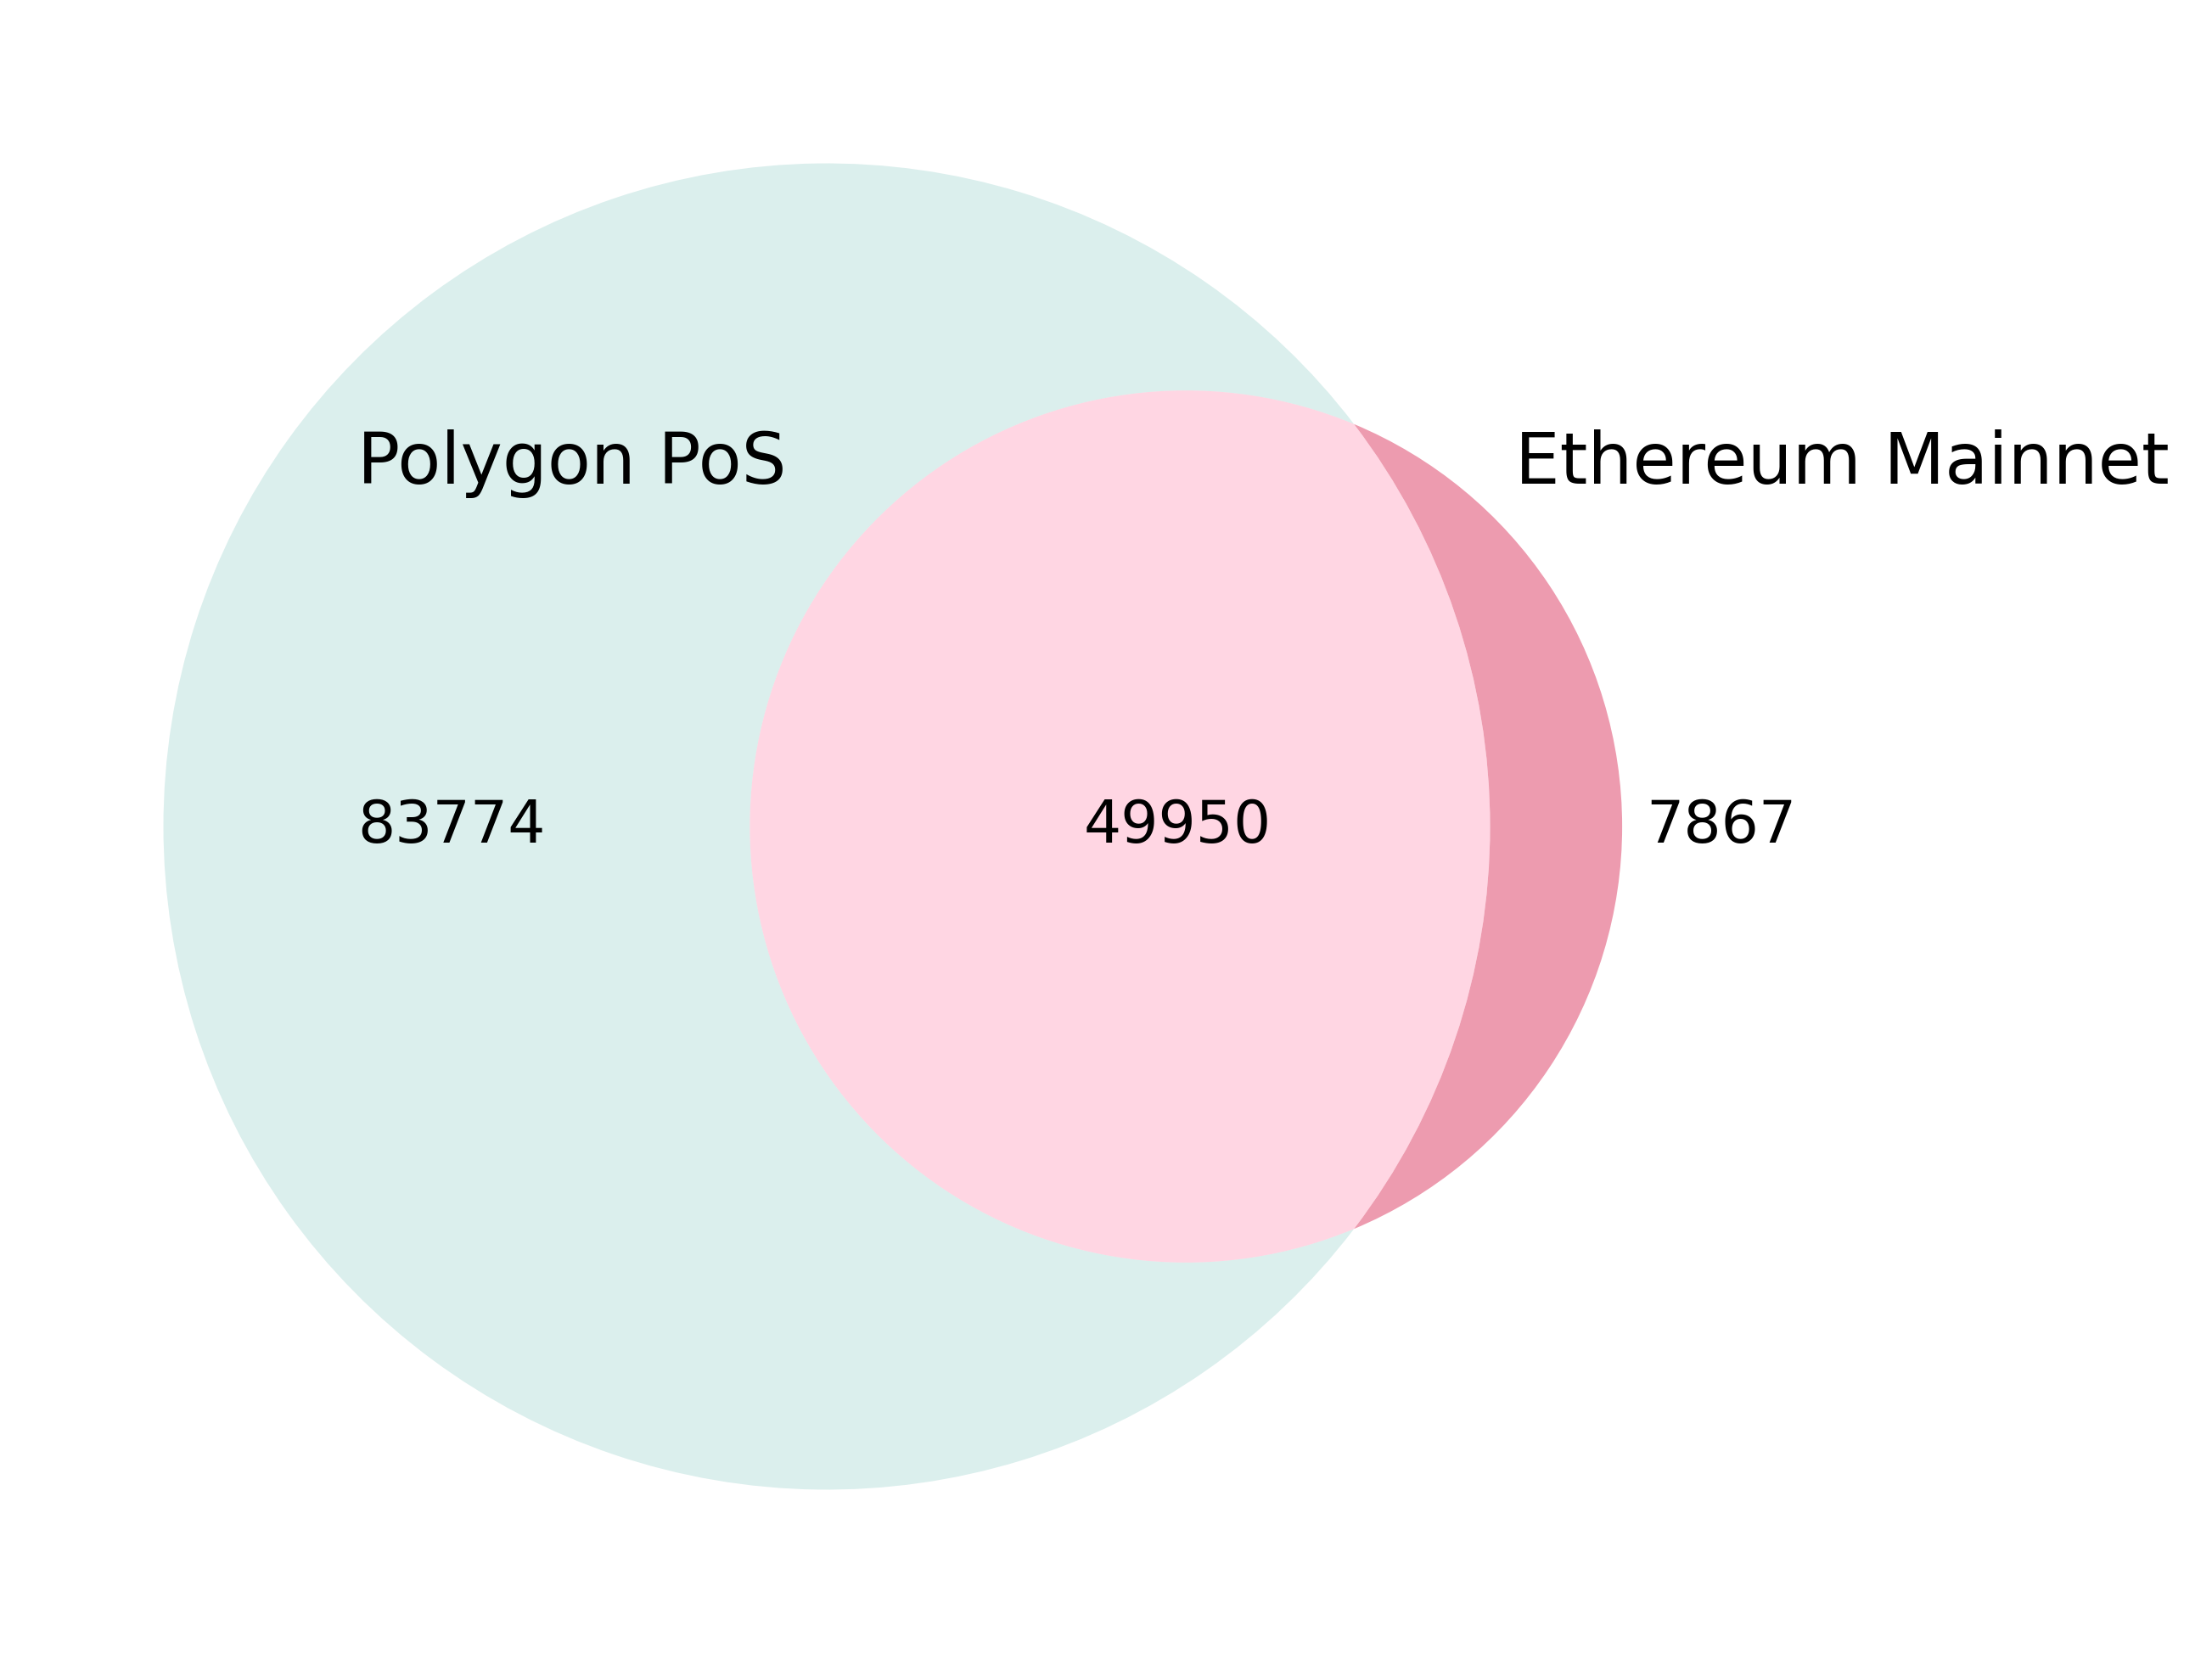
\includegraphics[width=0.6\textwidth]{../figures/venn_diagram.png}
	\caption{Venn Diagram of address subsets}
	\label{fig:Venn}
\end{figure} 

\subsection{Transactions and Token Transfer Events}
The address subsets were used to collect transaction and token transfer event data from Ethereum and Polygon. Ethereum or Polygon data can be accessed directly through a node or an application programming interface (API) provider like Infura or Etherscan. The absence of account indexing in Ethereum or Polygon poses a challenge for retrieving all past transactions and token transfers of a specific address, as it requires scanning through all blocks and token transfer events emitted by designated token contracts. Fortunately, Etherscan offers an API Endpoint Module for ``Accounts`` that facilitates the retrieval of transactions and token transfer events for a given address. By using our network-specific address subsets, we were able to significantly decrease the number of required API calls. 
We gathered all transactions and token transfers up until block \texttt{17,670,000} on Ethereum (July 11, 2023) and block \texttt{44,990,000} on Polygon (July 12, 2023). In total, we collected more than 30 million %30,689,978
token transfer events and more than 16 million %16,092,531
 normal transactions. While the amount of transactions is similar between the two networks, there are three times more transfer events on Polygon. \newline The output was stored in separate CSV files and also imported into a MongoDB\footnote{\url{https://www.mongodb.com/}} database.The database contains distinct collections for transactions and transfers. For information on the different data fields, see Appendix. 
 

\iffalse
Transfer Events: 30,689,978
Transfer Events Ethereum: 7,832,778
Transfer Events Polygon: 22,857,200

Transactions = 16,092,531
Transactions Ethereum = 8,448,584
Transactions Polygon = 7,643,947

Figure X visualizes the number of daily transactions and token transfers for each chain.
\begin{figure}[h!]
	\centering
	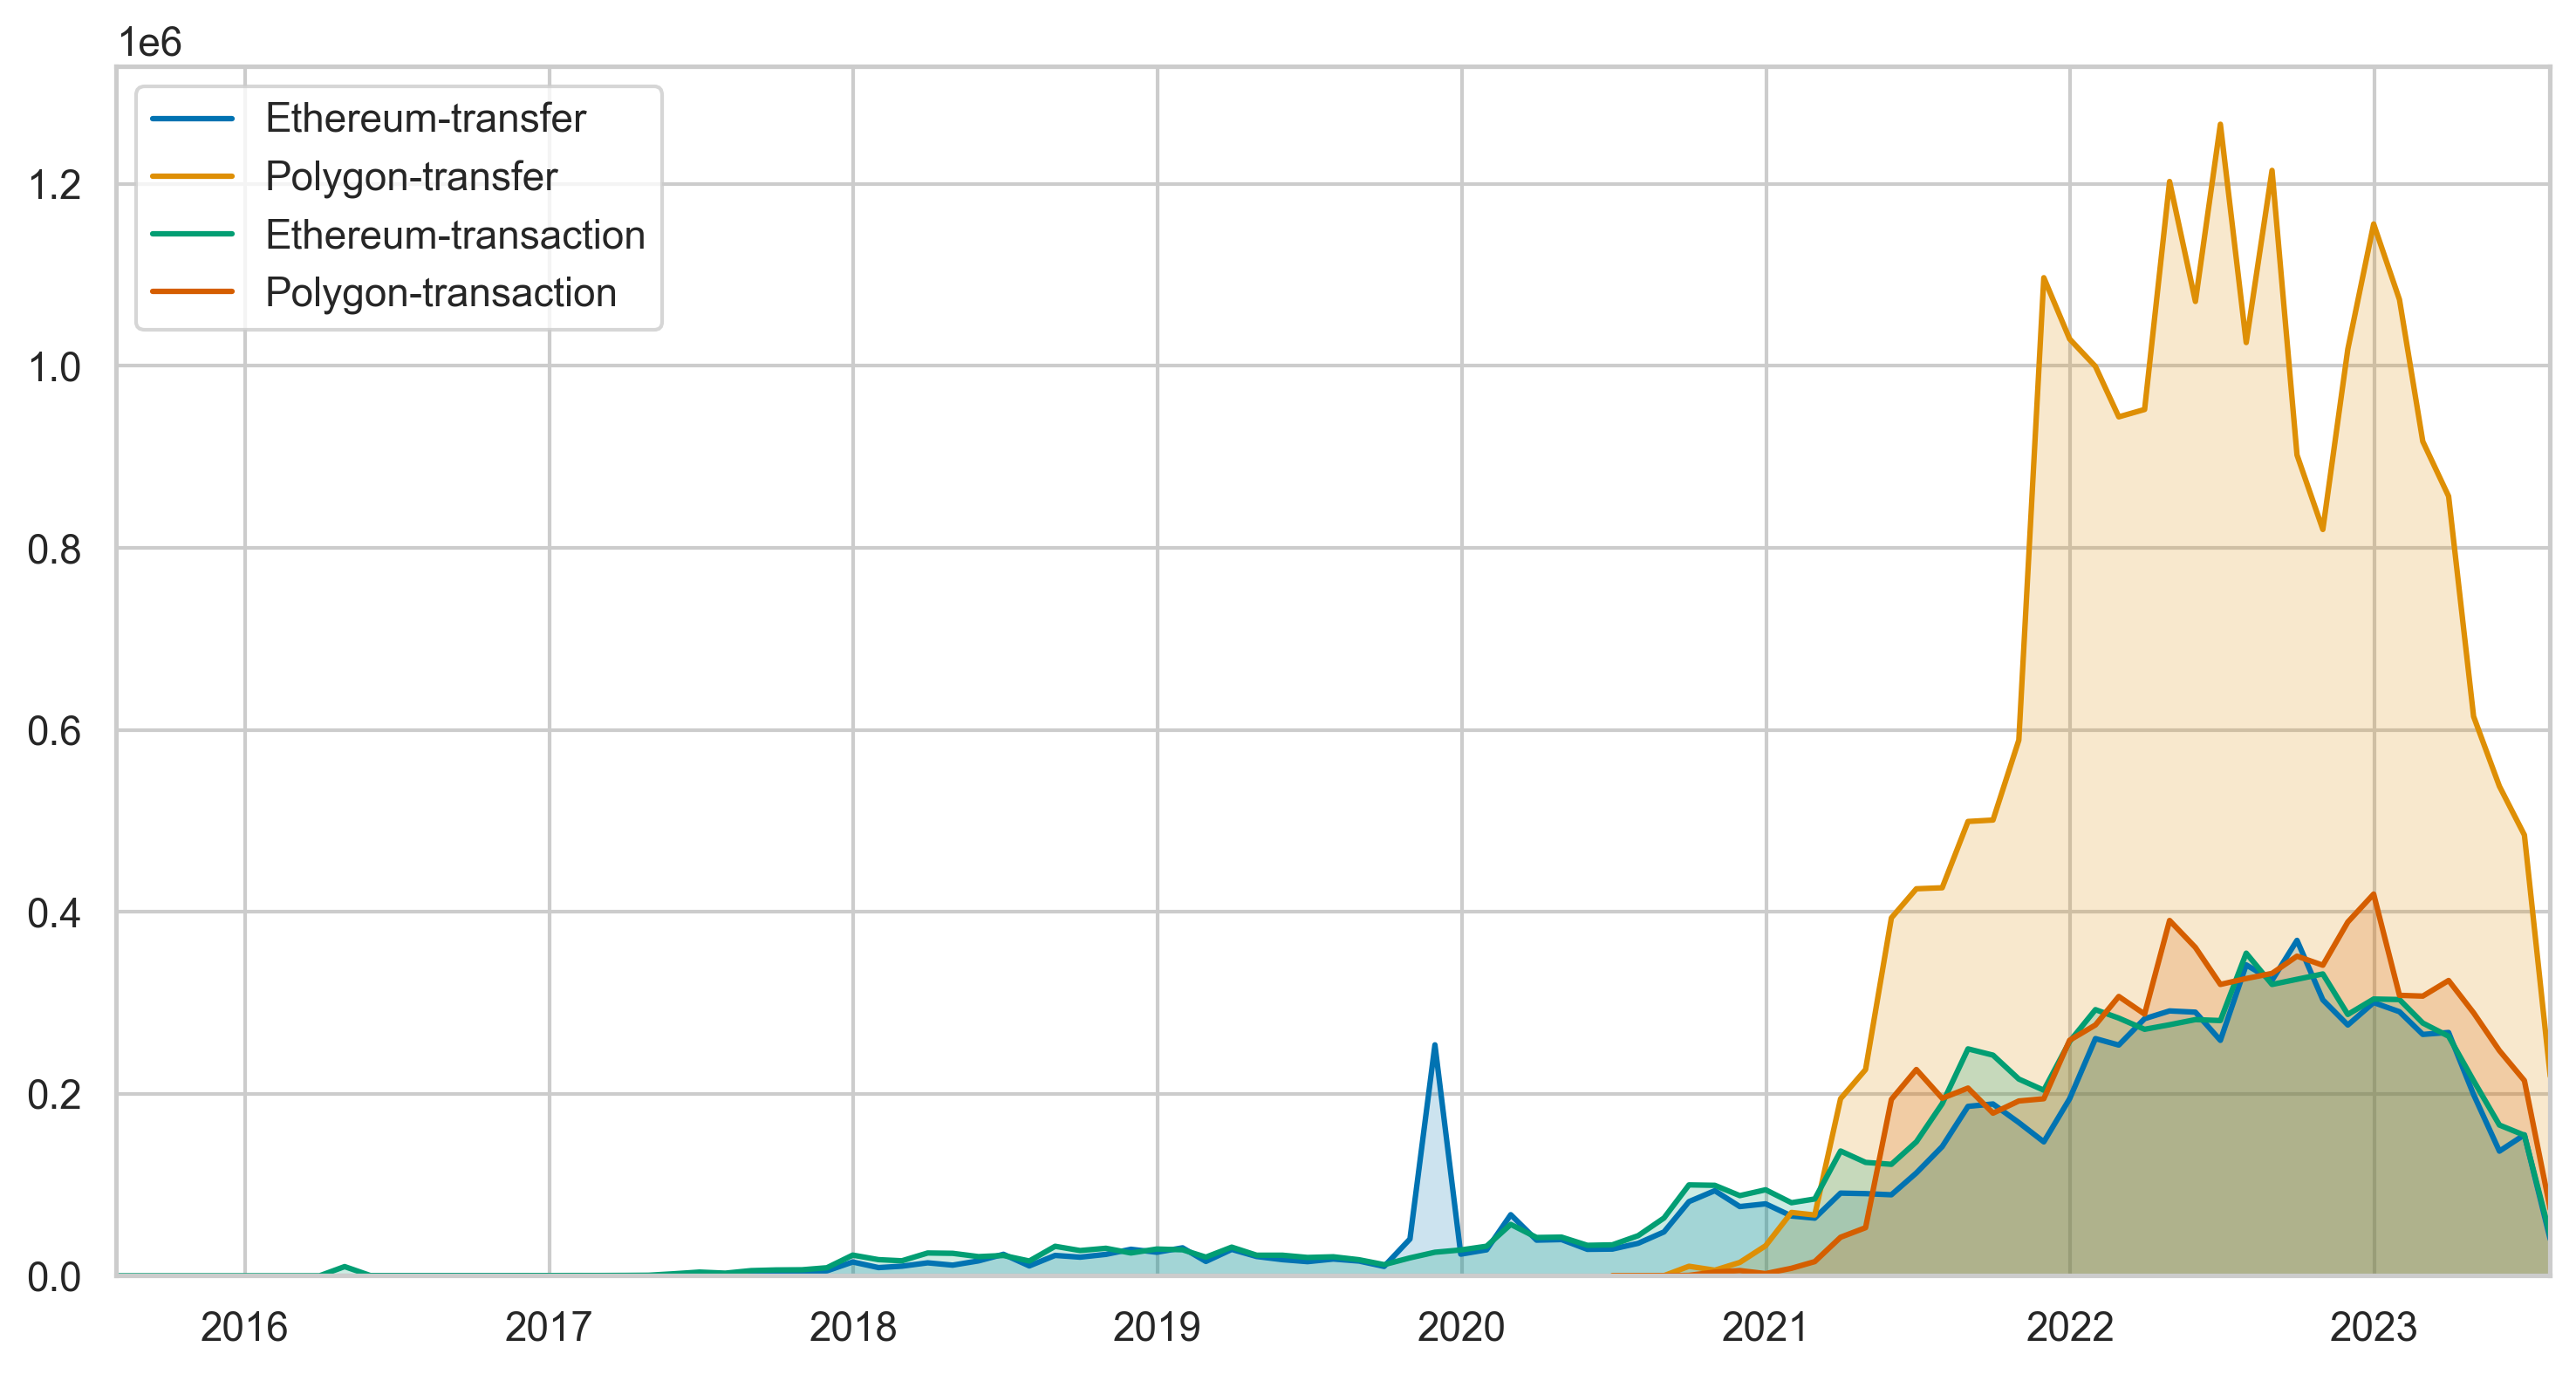
\includegraphics[width=\textwidth]{../figures/transfers_tx_by_chain.png}
	\caption{Monthly Transactions and Token Transfers by chain}
	\label{fig:Data}
\end{figure} 
Transfer Events, adding Information (isInSet) \\
Transactions \\
Filtering, Intra-set transfers\\
Data Structure, Fields \\
\fi


\subsection{Intra-set asset transfers}
In this project, we want to use entity clustering to determine the number of entities that are represented by the remaining 137,544 addresses. Or, to phrase it differently, do users interact with Decentraland using multiple EOAs, and can we identify addresses that belong to the same user?
\newline
To achieve this, we often only need to consider transactions or token transfer events where both the ``\texttt{from}`` (sender) and the ``\texttt{to}`` (recipient) address are within the address set. Regarding normal transactions, this means that we only keep native asset transfers (Ether or Matic) as almost all addresses are EOAs. \newline
The intra-set asset transfer dataset is mainly used to generate the network graphs (see section xx). When clustering addresses using graph-based approaches, this has the advantage that we do not need to differentiate between EOAs and smart contract account later on. Furthermore, it allows us to observe and visualize the asset flows between users. In total, we have 974,478 intra-set token transfers and 210,548 intra-set native asset transfers (101,621 Matic, 108,927 Ether).

\iffalse
%As nearly all addresses are Externally Owned Accounts (EOAs), we do not need to differentiate between EOAs and smart contract accounts, which further simplifies the clustering process. \newline
%(logging in to Decentraland with multiple addresses) When it comes to entity clustering, we essentially want to answer the question of how many real-world entities our remaining  137,544 addresses represent. 
-Also for other clustering heuristics we often make this reduction, for example: In the self-approval approach, we only consider approval transactions where another address from the set is approved.
-filter our transactions and token transfers to entries where both the 'from' and the 'to' are within this narrowed pool of addresses. We define this as intra-set asset transfers. For the transactions, this means that we only consider native asset (Ether or matic) transfers. %between two EOAs
-As already mentioned in the introduction, the goal of this paper is to cluster addresses within who (1) were active in Decentraland during the 9-month period (e.g., within the initial dataset) and (2) transacted or interacted with any token on Ethereum or Polygon. 
-Essentialy, we want to answer two main research questions when it comes to clustering:
1. How many unique entities does the address set represent (i.e. were active on Decentraland during the 9-month period)?
2. Are users interacting through multiple accounts/EOAs/addresses with Decentraland?
-we focus on on-chain data (and not user location or avatar data), allowing us to exclude addresses that have not transacted or interacted with any token on Ethereum or Polygon. 
-As mentioned in the introduction, the goal of this paper is to cluster addresses belongig to the same entity that were recorded/active in Decentraland during the 9-month period. Therefore, we disregard addresses outside of this set. Also, since we only look at on-chain data, we cannot cluster addresses without activity on Polygon or Ethereum. Doing these two reductions, there are  141, 591 'clusterable' addresses remaining.
-Since all of our addresses are EOAs (some multisig smart contract wallets). -> Check this?
\fi

\subsection{ENS ground-truth pairs}
Similarly to \cite{Beres2020}, we use Ethereum Name Service (ENS) identifiers as ground truth information to evaluate some of the clustering methods.\newline
\textit{ENS} is a naming system that relies on the Ethereum smart contracts. Its main purpose is to map human-readable names, such as \texttt{`alice.eth`}, to machine-readable identifiers, mostly Ethereum addresses. The architecture of ENS comprises two main components: the registry and resolvers. \newline
The \textit{ENS registry} consists of a single smart contract\footnote{The registry contract is ERC-721 compliant, which means that .eth registrations can be transferred in the same way as other NFTs.} that maintains a list of all domains and subdomains, recording the ``owner`` and ``resolver`` for each. The registry allows the owner of a domain to make changes to that data. \citep{ENSdocs} %Domain owners may set the resolver for the domain.
\newline
\textit{Resolvers} are responsible for %(the actual process of)
 translating names into addresses. Any contract that adheres to the relevant standards may act as a resolver. The process of resolving a name involves two steps: \textit{First}, the registry must be queried to find out which resolver is responsible for the name, and \textit{second}, that resolver must be asked for the response to the query. \newline
In addition to regular resolution from name to address, ENS also supports ``reverse resolution``, allowing for a mapping from address back to a name (or other metadata). Reverse resolution is accomplished via %special
 domain \texttt{`addr.reverse`}% and the resolver function \texttt{name()}.
. This domain is owned by a special purpose registrar contract that allocates subdomains to the owner of the matching address - for instance, the address \texttt{`0x1234\dots`} may claim the name \texttt{`1234\dots.addr.reverse`}, and configure a resolver and records on it. The resolver in turn supports the \texttt{name()} function, which returns the name associated with that address.\newline
 Reverse resolution %(without a library)
 follows the same pattern as forward resolution: Get the resolver for \texttt{`1234....addr.reverse'} (where \texttt{`1234...`} is the address you want to reverse-resolve), and call the \texttt{name()} function on that resolver. However, ENS does not enforce the accuracy of reverse records. This means \texttt{`1234....addr.reverse`} may falsely claim that the name associated to their address is \texttt{`alice.eth`}. 
 
Figure \ref{fig:ENS} illustrates the mechanism that allowed us to generate ground truth pairs in a simplified way: Initially, the domain name \texttt{`foo.eth`} resolves to address \texttt{`0xABC...`}. The owner has also set a reverse resolution for this address, indicated by the the edge from the address to the domain name. Next, the owner (he) decides to change the resolved address to \texttt{`0xDEF...`}. Again, he is setting a reverse record.  As a domain can only point to one address at the time, the previous mapping from address to old address is deleted. However, \texttt{`ABC....addr.reverse`} still points to \texttt{`foo.eth`} and when we query the name corresponding to \texttt{`0xABC...`} and \texttt{`0xDEF...`}, both will return \texttt{`foo.eth`}.
If this special case occurs, we assume that both addresses belong to the same entity.
%We did not observe cases where someone set a reverse record to a completely unrelated address (e.g. alice.eth)

\begin{figure*}[h!]
	\begin{center}
		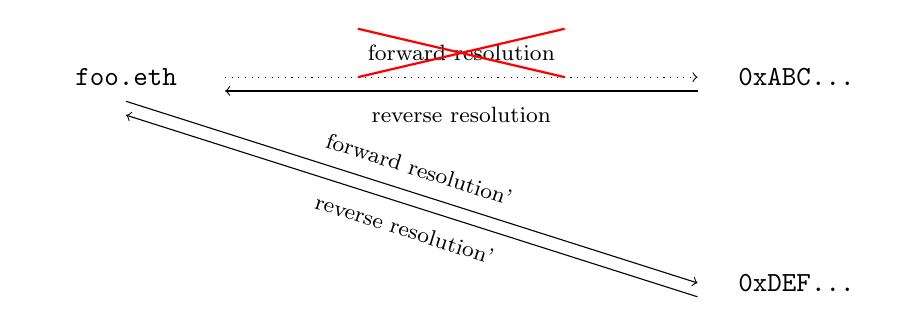
\begin{tikzpicture}[
    every node/.style={minimum width=2.5cm, minimum height=0.6cm, align=center},
    every path/.style={->},
    node distance=2cm and 6cm]

		\node (A) {\texttt{foo.eth}};
		\node[right=of A] (B) {\texttt{0xABC...}};
		\node[below=of B] (C) {\texttt{0xDEF...}};
		
		\draw[dotted] (A) -- (B) node[midway, above, name=pathAB] {\footnotesize{forward resolution}};
		\draw ([yshift=-5pt]B.west) -- ([yshift=-5pt]A.east) node[midway, below] {\footnotesize{reverse resolution}};
		\draw (A.south) -- (C.west) node[midway, sloped, above] {\footnotesize{forward resolution'}};
		\draw ([yshift=-5pt]C.west) -- ([yshift=-5pt]A.south) node[midway, sloped, below] {\footnotesize{reverse resolution'}}; 	
		
		% Adding a cross over "forward resolution"
        \draw[red, thick, -] (pathAB.south west) -- (pathAB.north east);
        \draw[red, thick, -] (pathAB.south east) -- (pathAB.north west);
							
		\end{tikzpicture}
		\caption{Changing the record to another address does not change the old reverse resolution (Simplified Schematic Representation)}
		\label{fig:ENS}
	\end{center}
\end{figure*}

We applied the following methodology to find ground truth pairs: First, we collected all addresses that interacted ENS (NFTs) to reduce the amount of name look-ups. For each of the remaining addresses, we checked if it points to an ENS domain name\footnote{This was done via the ENS module within web3.py \url{https://web3py.readthedocs.io/en/stable/ens_overview.html}}. If it did, we stored the associated ENS domain alongside the address in a CSV file. %(It provides an interface to look up domains and addresses). 
Using the newly generated list, we checked if two addresses point to the same ENS domain. If this check was met, we stored both addresses alongside the ENS domain. \newline
We found 11,440 reverse records and 40 address pairs. %(addresses pointing to the same .eth name)
We use these pairs as our ground truth to measure the performance of different clustering heuristics. Even though this is a small sample compared to the total number of 'clusterable' addresses, we should still be able to evaluate (compare) the methods and infer their efficacy. %profiling techniques


\iffalse
-Check for each address in the list if the address points to an human-readable name. (reverse mapping must be set/configured) From the web3.py documentation \url{https://web3py.readthedocs.io/en/stable/ens_overview.html } %The ens module is included with web3.py. It provides an interface to look up domains and addresses, add resolver records, or get and set metadata.
-If two addresses point to the same ENS name we consider them belonging to the same entity. 
-Normally, one .eth domain cannot point/map to multiple Ethereum addresses. Forward resolution. This is likely due to the owner change and the record not updated.

%However, if someone sets the forward resolution to a new address (owner) including a reverse resolution for his ENS name, the (reverse) resolution from 0x05d.addr.reverse still resolves to the the ENS domain name.
%Only the forward resolution from the name to the address is changed. The reverse record resolution from the old address to the name is still there. For an visual explanation please see Figure \ref{fig:ENS}.
%In addition to regular resolution from name to address, ENS also supports ``reverse resolution``, making it possible to map from address back to a name (or other metadata).
%Anyone who owns a domain at any level may configure subdomains - for themselves or others - as desired. For instance, if Alice owns 'alice.eth', she can create 'pay.alice.eth' and configure it as she wishes.
%Currently, all the subdomains or non .eth domains are not NFTs, unless the domain registrar itself supports NFT such as (dcl.eth, and .kred).
%If the owner sets a reverse resolution set with his new address, we have two addresses pointing to the same ens name. 

%While 'regular' resolution involves mapping from a name to an address, reverse resolution maps from an address back to a name - or other metadata. ENS supports reverse resolution to allow applications to display ENS names in place of hexadecimal addresses. Before this can be done, the owner of the address has to configure reverse resolution for their address.
%In spirit, it is similar to the well-known Domain Name Service (DNS). However, in ENS the registry is implemented in Ethereum smart contracts.
%Therefore, ENS provides a more user-friendly way of transferring assets on Ethereum, where users can use ENS names as recipient addresses instead of the error-prone hexadecimal Ethereum addresses.
%Resolving a name is a two-step process: First, ask the registry what resolver is responsible for the name, and second, ask that resolver for the answer to your query.\newline

\fi

%%%%%%%%%%%%%%%%%%%%%%%%%%%%%
%%% Clustering Heuristics %%%
%%%%%%%%%%%%%%%%%%%%%%%%%%%%%

\section{Clustering Heuristics}
In this section, we provide a overview of clustering heuristics in the context of account-based blockchains and on-chain data. We will give a detailed explanation of the intuition/rationale behind the heuristic, the workings and discuss the applicability for our case. In Section 5 we will then apply  and, if possible, evaluate the heuristics deemed suited for us.
%detailed explanation
% Goal: explain each heuristic, categorize, and discuss applicability to our address set

\subsection{Self-authorization}
\iffalse
	This heuristic was formulated in \cite{FV:17}. 
	All three token standards have/require functionality around approvals. These functions allow another address to spend tokens on behalf of the actual owners. This is mainly used in connection with smart contracts, but can also be applied for regular EOAs. Users could approve another address they own. Reasons for this might be risk distribution over several addresses with partial accessibility ...
		- approve(address,uint256)
		- setApprovalForAll(address,bool) for both ERC-721 and ERC-1155
		- safeBatchTransferFrom(address,address,uint256[],uint256[],bytes)
\fi

The \texttt{`approve`} function required in all three token standards allows another address to spend tokens on behalf of the actual owners. This functionality is mainly used in connection with smart contracts, but can also be applied for regular EOAs. Users could approve another address they own, a reason for this might be risk distribution over several addresses with partial accessibility. \citep{FV:17} 

Since we have all the addresses transactions, we can find transactions where someone approved another address from our set. 

The first step is to get all approval transactions. We achieve this using the 'input'/calldata field. The first X bytes are always the function selector. We filter for the known function selectors for all standards. Next, we get the approved address/spender, also from the calldata, it is always at the same spot. We filter for spenders within the address set and for spenders who are different from the 'from' address. How many transactions are remaining? 

\subsection{Deposit address reuse}
This heuristic exploits the common practice of crypto exchanges creating so-called deposit addresses for each user, which forward funds to a main address. Multiple addresses that send funds to the same deposit address are highly likely controlled by the same entity. \citep{FV:17}
We only have the addresses' transaction or token transfers, in order to get the exchange addresses, we would need to go one step further. -> We do not apply this with our dataset.

\subsection{Airdrop multi participation}
Airdrops are popular token distribution mechanisms, and recipients are mostly chosen based on past protocol activity. A famous example is Uniswap's UNI airdrop, where each address that interacted with the protocol received a fixed amount of UNI tokens\footnote{\url{https://blog.uniswap.org/uni}}. These distribution mechanisms are often not Sybil-resistant, leading to people creating multiple addresses in anticipation of an airdrop. However, managing the tokens on all of these addresses is impractical, which is why they are often aggregated into one address. \citep{FV:17}

\subsection{Graph-based network analysis}
Token networks -> Victor, Casale Brunet

%The set of addresses used in interactions characterize a users. Users with multiple accounts might interact with the same addresses from most of them. Furthermore, as users move funds between their personal addresses, they may unintetionally reveal their address clusters. Clustering experiments conducted on a transaction/transfer graph with nodes as addresses and edges as transactions/transfers. Rozemberczki provides a library of node embedding methods to discover address pairs that might belong to the same user. Preprocessing steps: transfers as undirected edges, remove loops and multi-edges, exlcude nodes outside the largest connected component. Resulting graph. Applied 3 node embedding methods to this graph (Diff2Vec, Role2Vec and deep walk.
\textbf{Node embeddings}

Projects addresses to points in a low-dimensional vector space based on who it interacts with. In this vector space, adresses belonging to the same entity should be close together in Euclidean distance.

Consider constructing an undirected graph from all Ethereum transactions where nodes are composed of distinct addresses, and an edge is placed between two nodes if there is a transaction between them.

At this abstraction layer, we seek to learn a ``node embedding function``that projects a node to a d-dimensional vector representation. Importantly I want this embedding to capture semantic information about the node, such as which other addresses it frequently interact with. To do so, we leverage popular graph representation learning algorithms. (Grover and Leskovec, 2016; Rozemberczki and Sarkar, 2018). In particular, we focus on Diff2Vec, Role2Vec and 


Given an address, to find its cluster, we can search for the closest k vectors in Rd. In practice, we accomplish this efficiently using FAISS (Johnson et al., 2019). This will always return k addresses.

Node embedding methods form a class of network representation learning methods that map graph nodes to vectors in a low-dimensional space. They are designed to represent vertices with similar neighborhood structure by vectors that are close in the vector space. Intuitively, addresses that interact with the same set of addresses in the Ethereum transaction graph should be close in the embedded space. Research in node embedding has been catalyzed by Word2Vec, an embedding method for natural language processing. 
... In this work, we use these techniques on the Ethereum transaction graph to link addresses owned by the same user.
...
The set of addresses used in interactions characterize a user. Users with multiple accounts might interact with the same addresses or services from most of the. Furthermore, they may unintentionally reveal their address clusters. Our deanonymization methods are conducted on a transaction graph with nodes as Ethereum addresses and edges as transactions. From the library of \cite
Diff2Vec, Role2Vec, DeepWalk \\
Transaction Graph Analysis

\subsection{Time-of-day transaction activity}
Transaction timestamps reveal the daily activity patterns of the account owner -> example
Given the set of timestamps, an account is represented by the vector including the mean, median and standard deviation, as well as the time-of-day activity histogram dividid into $b_{hour}$ bins. We chose 50 bins (from beres)

\subsection{Gas price distribution}
Gas price definition, often set by the wallet software (slow, medium, fast), given the changes in traffic volume we normalice the gas price bxy the daily network average in our dataset. Make example. Given the normalized gas prices of the transactions sent, an account is represented by the mean, median and standard deviation, as well as the normalized gas price histogram divided into $b_{gas}$ bins. We chose 6 bins (4 hour intervals) according to Beres.


\subsection{Own heuristics}



%%%%%%%%%%%%%%%%%%%%%
%%% Data Analysis %%%
%%%%%%%%%%%%%%%%%%%%%

\section{Data Analysis}




%%%%%%%%%%%%%%%%%%
%%% Discussion %%%
%%%%%%%%%%%%%%%%%%

\section{Discussion}



%%%%%%%%%%%%%%%%%%
%%% Conclusion %%%
%%%%%%%%%%%%%%%%%%

\section{Conclusion}



%%%%%%%%%%%%%%%%%%%%%%%%%%%%
%%% Literaturverzeichnis %%%
%%%%%%%%%%%%%%%%%%%%%%%%%%%%

\newpage
\setcounter{page}{1}
\pagenumbering{roman}
\onehalfspacing
\addcontentsline{toc}{section}{References}
\bibliography{mybib}
\bibliographystyle{agsm}

\section{Appendix}


Database



%% Table
\begin{table}[h!]
  \centering
  \footnotesize
  \begin{tabular}{l p{9cm} cc}
    \hline\hline
    Field & Description & Transfers & Transactions\\ \hline
    \texttt{hash} & Transaction hash & \checkmark & \checkmark \\
    \texttt{timeStamp} & Timestamp in seconds from the UNIX epoch & \checkmark & \checkmark \\
    \texttt{gasUsed} & Amount of gas used by the transaction & \checkmark & \checkmark \\
    \texttt{gasPrice} & Gas price specified for this transaction & \checkmark & \checkmark \\
    \texttt{nonce} &  \textbullet{ }EOAs: \newline \textbullet{ }CAs: & \checkmark & \checkmark \\
    \texttt{from} & \textbullet{ }Transactions: Address initiating the transaction\newline \textbullet{ }Transfers: Sender address & \checkmark & \checkmark \\
    \texttt{to} & \textbullet{ }The recipient's hexadecimal address. For transactions (native asset/token transfer or contract execution) \newline \textbullet{ }Transfers: Recipient address & \checkmark & \checkmark\\
    \texttt{value} &  \textbullet{ }Transactions: Amount of native asset sent \newline \textbullet{ }Transfers: Amount of token sent (\texttt{NaN} for NFTs)  & \checkmark & \checkmark\\
    \texttt{tokenID} &  Token identifier (\texttt{NaN} for ERC-20 tokens) & \checkmark & \\
    \texttt{input} & Calldata & Contract execution or deployment instructions & \checkmark \\
    \texttt{functionName} & Name of the function called, added by Etherscan / Polygonscan (\texttt{NaN} if not available) & \checkmark & \\
    \texttt{type} & Token standard. Created manually to combine token transfer events from different standards & \checkmark & \\
    \texttt{chainName} & Name of the blockchain. Created manually to combine Ethereum and Polygon data & \checkmark & \checkmark\\
    \hline\hline
  \end{tabular}
  \caption{Database Collection Fields}
  \label{tbl:database_schema}
\end{table}


Distinction: Transaction is a message sent from an externally owned account
((isSet, userAddress))
%%



\end{document}


%%% Table
%\begin{table}[h!]
%  \center
%  \begin{tabular}{lcc}
%    \hline\hline
%    Header & Header & Header \\ \hline
%    Entry 1 & $0 \leq x<1$ & $\alpha$\\
%    Entry 2 & $x=1$ & $\beta$\\
%    Entry 3 & $x>1$ & $\gamma$\\
%    \hline\hline
%  \end{tabular}
%  \caption{This is a table}
%  \label{tbl:test}
%\end{table}
%%%
